\begin{figure}[htbp] %  figure placement: here, top, bottom, or page
   \centering
   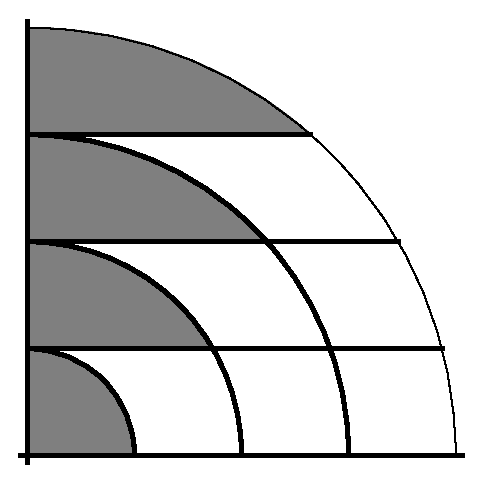
\includegraphics[ width = 1.5in ]{graphics/dominance_col.eps} \qquad
   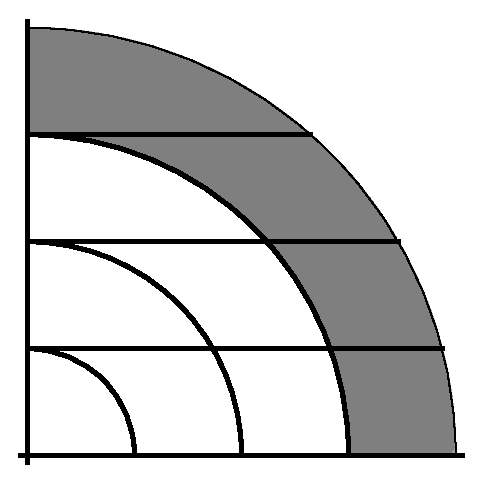
\includegraphics[ width = 1.5in ]{graphics/dominance_band.eps} \\
   (a) $A_{\Lambda,1}$,  theorem \eqref{eq:limb dom}  \qquad  \qquad  \qquad
   (b) $A_{k,k}$,  theorem \eqref{eq:shell dom} \\
   $A_{1,1} > A_{2,1} > A_{3,1} > \cdots A_{n,1}$ \qquad
   $A_{1,1} > A_{2,2} > A_{3,3} > \cdots A_{n,n}$
   \caption{Two dominance schemes will help to quantify the behavior of the system matrix $\B$ to be introduced in section \eqref{sec:b matrix}.}
   \label{fig:hierarchies}
\end{figure}

\endinput
